\section{Service Description}
\label{sec:serv_desc}

The Remote SmartHouse Control (RSHC) Protocol serves as a communication mechanism between a client device and server. Built to communicate between a SmartHouse Controller and a remote device, RSHC provides the capability to manipulate devices within the home by interacting with the SmartHouse server, which in turn is responsible for communications with the devices themselves. Though the ability to communicate with household devices is left to the SmartHouse server, RSHC's sole purpose is to translate the actions the client would like to perform to the server so that they may be carried out.


To further explain this relationship, provided is Figure \figr{fig:serv_desc:service} which shows the direct location of the protocol in relation to the overall SmartHouse schema.

\begin{figure}[h]
  \centering
  \label{fig:serv_desc:service}
  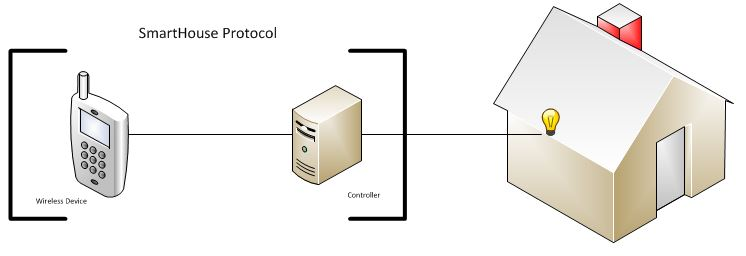
\includegraphics[width=5in]{figures/desc_img.jpg}\\
  \caption{Protocol interaction diagram.}
\end{figure}

RSHC is independent of a transmission subsystem and requires a reliable ordered data stream channel without fixed size boundaries for transport, for which TCP/IP is the optimum choice for this discussion. An important security feature of RSHC is the use of DES Authentication for the initial authorization of the client device. Although no encryption is provided throughout, the ability to transmit over SSL is a possible option.
